\lhead[\thepage]{CHAPTER \thechapter. VERIFICATION, VALIDATION AND EVALUATION}
\chead[]{}
\rhead[A Complete Simulator for Volunteer Computing Environments\leftmark]{\thepage}
\renewcommand{\headrulewidth}{0.5pt}

\lfoot[]{}
\cfoot[]{}
\rfoot[]{}
\renewcommand{\footrulewidth}{0pt}

%% This is an example first chapter.  You should put chapter/appendix that you
%% write into a separate file, and add a line \include{yourfilename} to
%% main.tex, where `yourfilename.tex' is the name of the chapter/appendix file.
%% You can process specific files by typing their names in at the 
%% \files=
%% prompt when you run the file main.tex through LaTeX.
\chapter{Verificación, validación y evaluación}
\label{ch:verification_validation_and_evaluation}
\markboth{}{VERIFICATION, VALIDATION AND EVALUATION}

This chapter details the verification, validation and evaluation of the project. First, we present the verification and validation of the simulator (Section \ref{sec:verification_and_validation}, \textit{\nameref{sec:verification_and_validation}}), and we detail a series of tests that allowed us to verify that we had met all the requirements set in Chapter \ref{ch:analysis} (\textit{\nameref{ch:analysis}}). After this, we show the validation of the outputs of the simulations, demonstrating that the simulator performs accurate and realistic simulations. We also display a study of the performance of the simulator (Section \ref{sec:performance_study}, \textit{\nameref{sec:performance_study}}), in which we show that \gls{comsimboinc} is efficient and scalable. Finally, we present several case studies of the simulator usage (Section \ref{sec:case_studies}, \textit{\nameref{sec:case_studies}}), with the corresponding analysis and evaluation of the results.

We have used the drand48 Linux functions \cite{drand48} as random number generator in our simulations. These functions generate pseudo-random numbers using the linear congruential algorithm and 48-bit integer arithmetic. Each simulation result presented in this chapter is based on the average of 20 runs. For a 95\% interval, the error is less than $\pm$ 3\% for all values.

\section{Verificación y validación}
\label{sec:verification_and_validation}

The main objective of this section is to verify that all the requirements set out in Chapter \ref{ch:analysis} (\textit{\nameref{ch:analysis}}) have been fulfilled. In addition, we validate the results provided by \gls{comsimboinc}, comparing them to the results of SimBOINC and to the statistical results of the official \gls{boinc} webpage.

In software engineering, verification and validation are the processes of checking that a software system meets specifications and that it fulfills its intended purpose. As explained in Chapter \ref{ch:analysis} (\textit{\nameref{ch:analysis}}), the customer initially sets the requirements desired for the final product (user requirements). From there, analysts specify software requirements (functional and non-functional requirements). In order to verify that the project requirements are met, verification and validation processes are needed (see Figure \ref{fig:verification_validation}).

\vspace{1cm}

\begin{figure}[htb]
 	\centering
 	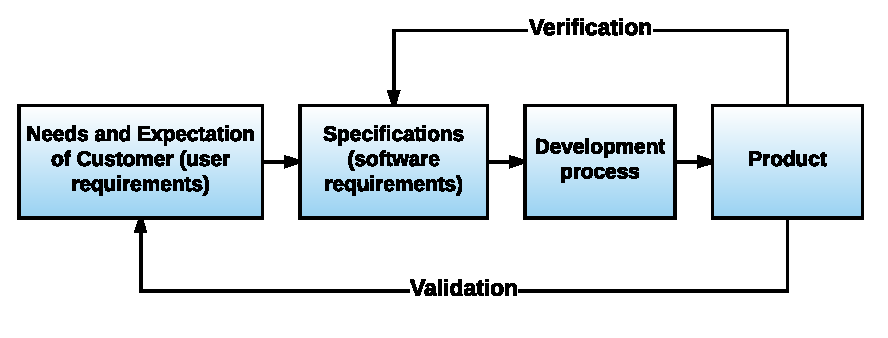
\includegraphics[width=12cm]{figures/verification_validation}
 	\caption{Software verification and validation.}
	\label{fig:verification_validation}
\end{figure}

\vspace{1cm}

\textit{Software verification} is the process of evaluating work-products (not the actual final product) of a development phase to determine whether they meet the specified requirements for that phase (the software requirements). \textit{Software validation} is the process of evaluating the final product at the end of the development process to determine whether it satisfies the requirements specified by the user at the beginning of the project \cite{verification}.


\subsection{Pruebas de verificación}

In order to perform the verification tests, we have followed a dynamic process during the development phase of the software. With these tests we wanted to answer the question: ``Are we building the product right?''. Table \ref{tab:verification_tests} provides the template used for the verification tests. Note that the ID format is VET-XX, where XX indicates the verification test number.

\clearpage

\begin{center}
\begin{table*}[htb]
\centering
\begin{tabular}{@{}p{2.5cm} p{9cm}@{}} 
\toprule
\textbf{ID} 					& Test ID. \\
\midrule
\textbf{Name} 				& Test name. \\
\midrule
\textbf{Requirements} 		& Software requirements fulfilled with this test. \\
\midrule
\textbf{Description} 		& Test description. \\
\midrule
\textbf{Preconditions}		& Predicates that must always be true before performing the test. \\
\midrule
\textbf{Procedure}			& A fixed, step-by-step sequence of activities performed by the test. \\
\midrule
\textbf{Postconditions} 		& Predicates that must always be true just after performing the test. \\
\midrule
\textbf{Evaluation} 			& \textit{Passed} or \textit{Failed}. \\
\bottomrule
\end{tabular}
\caption{Template for verification tests.}
\label{tab:verification_tests}
\end{table*}
\end{center}

Then, we specify the verification tests.

\vspace{0.7cm}

\begin{center}
\begin{table*}[htb]
\centering
\begin{tabular}{@{}p{2.5cm} p{13cm}@{}} 
\toprule
\textbf{ID} 					& VET-01 \\
\midrule
\textbf{Name} 				& Platform. \\
\midrule
\textbf{Requirements} 		& SR-NF-PL01, SR-NF-PL02, SR-NF-PL03, SR-NF-UI02. \\
\midrule
\textbf{Description} 		& Verify that the software can be used on the platform and is developed with the tools specified in the requirements. \\
\midrule
\textbf{Preconditions}		& 1. Use a machine with Ubuntu 14.04 operating system.\\
							& 2. GCC (GNU Compiler) 5.1 or higher must be installed on the machine. \\
							& 3. The user must be located in the main directory of the \gls{comsimboinc} application. \\
\midrule
\textbf{Procedure}			& 1. Check the code of the simulator source files (all these files are inside the /Files folder). \\
							& 2. Run the generator script with the default parameters to create the simulation files.\\
							& 3. Run the simulation.\\
\midrule
\textbf{Postconditions} 		& 1. All source files must be written in C programming language.\\
							& 2. The implementation, setup and control of the simulations must be carried out using the MSG API of the SimGrid toolkit.\\
							& 3. Simulations run while a progress bar indicates the percentage of execution. \\			
							& 4. The simulator must successfully finish its execution in the specified operating system. \\
\midrule
\textbf{Evaluation} 			& Passed \\
\bottomrule
\end{tabular}
\caption{Verification test VET-01.}
\label{tab:vet01}
\end{table*}
\end{center}


\begin{center}
\begin{table*}[htb]
\centering
\begin{tabular}{@{}p{2.5cm} p{13cm}@{}} 
\toprule
\textbf{ID} 					& VET-02 \\
\midrule
\textbf{Name} 				& Realistic BOINC elements in simulations. \\
\midrule
\textbf{Requirements} 		& SR-F-F06, SR-NF-UI01, SR-NF-UI02. \\
\midrule
\textbf{Description} 		& Verify that the simulator allows to simulate all the BOINC actual elements. \\
\midrule
\textbf{Preconditions}		& 1. The user must be located in the main directory of the \gls{comsimboinc} application.\\
\midrule
\textbf{Procedure}			& 1. Specify the following elements in the simulation parameters: tasks, volunteer hosts, servers, data servers, networks, and hosts availability.\\
							& 2. Run the generator script to create the simulation files.\\
							& 3. Run the simulation. \\
\midrule
\textbf{Postconditions} 		& 1. Simulations run while a progress bar indicates the percentage of execution. \\		
							& 2. The simulator must successfully finish its execution. \\
\midrule
\textbf{Evaluation} 			& Passed \\
\bottomrule
\end{tabular}
\caption{Verification test VET-02.}
\label{tab:vet02}
\end{table*}
\end{center}


\begin{center}
\begin{table*}[htb]
\centering
\begin{tabular}{@{}p{2.5cm} p{13cm}@{}} 
\toprule
\textbf{ID} 					& VET-03 \\
\midrule
\textbf{Name} 				& Statistics of BOINC projects. \\
\midrule
\textbf{Requirements} 		& SR-F-F02, SR-NF-UI01, SR-NF-UI02. \\
\midrule
\textbf{Description} 		& Verify that the outputs of the simulator are the same as those published by BOINCstats \cite{BOINC2016}. The outputs are: credits, hosts, active hosts, and \acrshort{flops}.\\
\midrule
\textbf{Preconditions}		& 1. The user must be located in the main directory of the \gls{comsimboinc} application. \\
\midrule
\textbf{Procedure}			& 1. Specify the simulation parameters.\\
							& 2. Run the generator script to create the simulation files.\\
							& 3. Run the simulation.\\
\midrule
\textbf{Postconditions} 		& 1. Simulations run while a progress bar indicates the percentage of execution. \\
							& 2. The simulator must successfully finish its execution. \\
							& 3. The outputs of the simulator contain at least: credits, hosts, active hosts, and \acrshort{flops} (The same as those published by BOINCstats \cite{BOINC2016}). \\
\midrule
\textbf{Evaluation} 			& Passed \\
\bottomrule
\end{tabular}
\caption{Verification test VET-03.}
\label{tab:vet03}
\end{table*}
\end{center}


\begin{center}
\begin{table*}[htb]
\centering
\begin{tabular}{@{}p{2.5cm} p{13cm}@{}} 
\toprule
\textbf{ID} 					& VET-04 \\
\midrule
\textbf{Name} 				& Multiple BOINC proyects simultaneously. \\
\midrule
\textbf{Requirements} 		& SR-F-F04, SR-NF-UI01, SR-NF-UI02. \\
\midrule
\textbf{Description} 		& Verify that the simulator allows multiple project simulations simultaneously. \\
\midrule
\textbf{Preconditions}		& 1. The user must be located in the main directory of the \gls{comsimboinc} application. \\
\midrule
\textbf{Procedure}			& 1. Specify the simulation parameters of three different projects (for example, the SETI@home, Einstein@home, and LHC@home projects).\\
							& 2. Run the generator script to create the simulation files.\\
							& 3. Run the simulation.\\
\midrule
\textbf{Postconditions} 		& 1. Simulations run while a progress bar indicates the percentage of execution. \\
							& 2. The simulator must successfully finish its execution. \\
\midrule
\textbf{Evaluation} 			& Passed \\
\bottomrule
\end{tabular}
\caption{Verification test VET-04.}
\label{tab:vet04}
\end{table*}
\end{center}


\begin{center}
\begin{table*}[htb]
\centering
\begin{tabular}{@{}p{2.5cm} p{13cm}@{}} 
\toprule
\textbf{ID} 					& VET-05 \\
\midrule
\textbf{Name} 				& BOINC client scheduler. \\
\midrule
\textbf{Requirements} 		& SR-F-F05, SR-NF-UI01, SR-NF-UI02. \\
\midrule
\textbf{Description} 		& Verify that the client scheduler implemented produces the same results as the actual BOINC scheduler. \\
\midrule
\textbf{Preconditions}		& 1. The user must be located in the main directory of the \gls{comsimboinc} application. \\
\midrule
\textbf{Procedure}			& 1. Specify the client side simulation parameters of three different projects: SETI@home, Einstein@home, and LHC@home. \\
							& 2. Run the generator script to create the simulation files.\\
							& 3. Run the simulation.\\
\midrule
\textbf{Postconditions} 		& 1. Simulations run while a progress bar indicates the percentage of execution. \\
							& 2. The simulator must successfully finish its execution. \\
							& 3. The outputs of the simulation are the same as the real BOINC client scheduler (it is detailed in \ref{subsec:validation_of_the_client_scheduler}, \textit{\nameref{subsec:validation_of_the_client_scheduler}}).  \\
\midrule
\textbf{Evaluation} 			& Passed \\
\bottomrule
\end{tabular}
\caption{Verification test VET-05.}
\label{tab:vet05}
\end{table*}
\end{center}


\begin{center}
\begin{table*}[htb]
\centering
\begin{tabular}{@{}p{2.5cm} p{13cm}@{}} 
\toprule
\textbf{ID} 					& VET-06 \\
\midrule
\textbf{Name} 				& Accurate simulations of BOINC projects. \\
\midrule
\textbf{Requirements} 		& SR-F-F01, SR-F-F03, SR-NF-UI01, SR-NF-UI02. \\
\midrule
\textbf{Description} 		& Verify that the outputs of the simulator for existing projects (SETI@home, Einstein@home, and LHC@home) should be almost identical to those published in BOINCstats \cite{BOINC2016}. \\
\midrule
\textbf{Preconditions}		& 1. The user must be located in the main directory of the \gls{comsimboinc} application. \\
\midrule
\textbf{Procedure}			& 1. Specify the simulation parameters of three different projects: SETI@home, Einstein@home, and LHC@home. \\
							& 2. Run the generator script to create the simulation files.\\
							& 3. Run the simulation.\\
\midrule
\textbf{Postconditions} 		& 1. Simulations run while a progress bar indicates the percentage of execution. \\
							& 2. The simulator must successfully finish its execution. \\
							& 3. The outputs of the simulation are the same as the actual BOINC projects, in terms of \acrshort{flops} and credit (it is detailed in \ref{subsec:validation_of_the_whole_simulator}, \textit{\nameref{subsec:validation_of_the_whole_simulator}}). \\
\midrule
\textbf{Evaluation} 			& Passed \\
\bottomrule
\end{tabular}
\caption{Verification test VET-06.}
\label{tab:vet06}
\end{table*}
\end{center}


\begin{center}
\begin{table*}[htb]
\centering
\begin{tabular}{@{}p{2.5cm} p{13cm}@{}} 
\toprule
\textbf{ID} 					& VET-07 \\
\midrule
\textbf{Name} 				& Large simulations. \\
\midrule
\textbf{Requirements} 		& SR-NF-S01, SR-NF-UI01, SR-NF-UI02. \\
\midrule
\textbf{Description} 		& Verify the application is able to perform simulations
with more than 100,000 hosts in a machine with at least 8 GB of \gls{ram}. \\
\midrule
\textbf{Preconditions}		& 1. Use a machine with at least 8GB or \gls{ram}. \\
							& 2. The user must be located in the main directory of the \gls{comsimboinc} application. \\
\midrule
\textbf{Procedure}			& 1. Specify the simulation parameters with more than 100,000 hosts. \\
							& 2. Run the generator script to create the simulation files.\\
							& 3. Run the simulation.\\
\midrule
\textbf{Postconditions} 		& 1. Simulations run while a progress bar indicates the percentage of execution. \\
							& 2. The simulator must successfully finish its execution. \\
\midrule
\textbf{Evaluation} 			& Passed \\
\bottomrule
\end{tabular}
\caption{Verification test VET-07.}
\label{tab:vet07}
\end{table*}
\end{center}


\begin{center}
\begin{table*}[htb]
\centering
\begin{tabular}{@{}p{2.5cm} p{13cm}@{}} 
\toprule
\textbf{ID} 					& VET-08 \\
\midrule
\textbf{Name} 				& Execution time. \\
\midrule
\textbf{Requirements} 		& SR-NF-P01, SR-NF-UI01, SR-NF-UI02. \\
\midrule
\textbf{Description} 		& Check that simulations follow a linear execution time. \\
\midrule
\textbf{Preconditions}		& 1. The user must be located in the main directory of the \gls{comsimboinc} application. \\
\midrule
\textbf{Procedure}			& 1. Specify the simulation parameters with different workloads. \\
							& 2. Run the generator script to create the simulation files.\\
							& 3. Run the simulation.\\
							
							& 4. Go to 2 specifying different simulation parameters.\\
\midrule
\textbf{Postconditions} 		& 1. Simulations run while a progress bar indicates the percentage of execution. \\
							& 2. The simulator must successfully finish its execution. \\
							& 3. Check that executions follow a linear execution time when increasing the workload (it is detailed in \ref{sec:performance_study}, \textit{\nameref{sec:performance_study}}). \\
\midrule
\textbf{Evaluation} 			& Passed \\
\bottomrule
\end{tabular}
\caption{Verification test VET-08.}
\label{tab:vet08}
\end{table*}
\end{center}


\clearpage


The verification test traceability matrix (Table \ref{tab:verification_matrix}) determines that all the software requirements have been verified during the development phase of the project.

\vspace{2cm}


\begin{table}[htb]
\ra{1.3}
  \centering
  \begin{tabular}{@{}L{3cm}C{0.7cm}C{0.7cm}C{0.7cm}C{0.7cm}C{0.7cm}C{0.7cm}C{0.7cm}C{0.7cm}@{}}
    \toprule
     \thead{Requirements} & \rothead{VET-01} & \rothead{VET-02} & \rothead{VET-03} & \rothead{VET-04} & \rothead{VET-05} & \rothead{VET-06} & \rothead{VET-07} & \rothead{VET-08}\\
    \midrule
    SR-F-F01 & & & & & & \ding{51} & &\\
    SR-F-F02 & & & \ding{51} & & & & &\\
    SR-F-F03 & & & & & & \ding{51} & &\\
    SR-F-F04 & & & & \ding{51} & & & &\\
    SR-F-F05 & & & & & \ding{51} & & &\\
    SR-F-F06 & & \ding{51} & & & & & &\\
    SR-NF-PL01 & \ding{51} & & & & & & & \\
    SR-NF-PL02 & \ding{51} & & & & & & &\\
    SR-NF-PL03 & \ding{51} & & & & & & &\\
    SR-NF-S01 & & & & & & & \ding{51} &\\
    SR-NF-P01 & & & & & & & & \ding{51}\\
    SR-NF-UI01 & & \ding{51} & \ding{51} & \ding{51} & \ding{51} & \ding{51} & \ding{51} & \ding{51}\\
    SR-NF-UI02 & \ding{51} & \ding{51} & \ding{51} & \ding{51} & \ding{51} & \ding{51} & \ding{51} & \ding{51}\\
    \bottomrule
\end{tabular}
\caption{Verification test traceability matrix.}
\label{tab:verification_matrix}
\end{table}    

\clearpage

\subsection{Validation Tests}

To perform the validation tests, we have checked the final software, comparing it with the user needs specified in Chapter \ref{ch:analysis} (\textit{\nameref{ch:analysis}}). With these tests we want to answer the question: ``Have we built the right product?''. Table \ref{tab:validation_tests} provides the template used for the validation tests. Note that the ID format is VAT-XX, where XX indicates the validation test number.

\begin{center}
\begin{table*}[htb]
\centering
\begin{tabular}{@{}p{2.5cm} p{9cm}@{}} 
\toprule
\textbf{ID} 					& Test ID. \\
\midrule
\textbf{Name} 				& Test name. \\
\midrule
\textbf{Requirements} 		& User requirements fulfilled with this test. \\
\midrule
\textbf{Verification tests} 	& Verification tests that help us to validate this test. \\
\midrule
\textbf{Description} 		& Test description. \\
\midrule
\textbf{Preconditions}		& Predicates that must always be true before performing the test. \\
\midrule
\textbf{Procedure}			& A fixed, step-by-step sequence of activities performed by the test. \\
\midrule
\textbf{Postconditions} 		& Predicates that must always be true just after performing the test. \\
\midrule
\textbf{Evaluation} 			& \textit{Passed} or \textit{Failed}. \\
\bottomrule
\end{tabular}
\caption{Template for validation tests.}
\label{tab:validation_tests}
\end{table*}
\end{center}


Then, we specify the validation tests.


\begin{center}
\begin{table*}[htb]
\centering
\begin{tabular}{@{}p{2.5cm} p{13cm}@{}} 
\toprule
\textbf{ID} 					& VAT-01 \\
\midrule
\textbf{Name} 				& BOINC projects simulation. \\
\midrule
\textbf{Requirements} 		& UR-C01. \\
\midrule
\textbf{Verification tests} 	& VET-03, VET-06. \\
\midrule
\textbf{Description} 		& Validate that the simulator is able to simulate the behavior of BOINC projects. \\
\midrule
\textbf{Preconditions}		&  1. The user must be located in the main directory of the \gls{comsimboinc} application. \\
\midrule
\textbf{Procedure}			& 1. Specify the simulation parameters of three different BOINC projects: SETI@home, Einstein@home, and LHC@home. \\
							& 2. Run the generator script to create the simulation files. \\
							& 3. Run the simulation. \\ 
\midrule
\textbf{Postconditions} 		& 1. The simulator must successfully finish its execution. \\
							& 2. The outputs of the simulation are the same as the actual BOINC projects, in terms of \acrshort{flops} and credit (it is detailed in \ref{subsec:validation_of_the_whole_simulator}, \textit{\nameref{subsec:validation_of_the_whole_simulator}}). \\
\midrule
\textbf{Evaluation} 			& Passed. \\
\bottomrule
\end{tabular}
\caption{Validation test VAT-01.}
\label{tab:vat-01}
\end{table*}
\end{center}


\begin{center}
\begin{table*}[htb]
\centering
\begin{tabular}{@{}p{2.5cm} p{13cm}@{}} 
\toprule
\textbf{ID} 					& VAT-02 \\
\midrule
\textbf{Name} 				& Client \gls{scheduling}. \\
\midrule
\textbf{Requirements} 		& UR-C02. \\
\midrule
\textbf{Verification tests} 	& VET-05. \\
\midrule
\textbf{Description} 		& Validate that the client scheduler implemented produces the same results as the actual BOINC scheduler. \\
\midrule
\textbf{Preconditions}		&  1. The user must be located in the main directory of the \gls{comsimboinc} application. \\
\midrule
\textbf{Procedure}			& 1. Specify the client side simulation parameters of three different projects: SETI@home, Einstein@home, and LHC@home. \\
							& 2. Run the generator script to create the simulation files. \\
							& 3. Run the simulation. \\ 
\midrule
\textbf{Postconditions} 		& 1. The simulator must successfully finish its execution. \\
							& 2. The outputs of the simulation are the same as the real BOINC client scheduler (it is detailed in \ref{subsec:validation_of_the_client_scheduler}, \textit{\nameref{subsec:validation_of_the_client_scheduler}}). \\
\midrule
\textbf{Evaluation} 			& Passed. \\
\bottomrule
\end{tabular}
\caption{Validation test VAT-02.}
\label{tab:vat-02}
\end{table*}
\end{center}


\begin{center}
\begin{table*}[htb]
\centering
\begin{tabular}{@{}p{2.5cm} p{13cm}@{}} 
\toprule
\textbf{ID} 					& VAT-03 \\
\midrule
\textbf{Name} 				& Simulation components. \\
\midrule
\textbf{Requirements} 		& UR-C03. \\
\midrule
\textbf{Verification tests} 	& VET-02. \\
\midrule
\textbf{Description} 		& Validate that the simulations cover all the elements of the BOINC infrastructure. \\
\midrule
\textbf{Preconditions}		&  1. The user must be located in the main directory of the ComBoS application. \\
\midrule
\textbf{Procedure}			& 1. Specify the following elements in the simulation parameters: tasks, volunteer hosts, servers, data servers, networks, and hosts availability. \\
							& 2. Run the generator script to create the simulation files. \\
							& 3. Run the simulation. \\ 
\midrule
\textbf{Postconditions} 		& 1. The simulator must successfully finish its execution. \\
\midrule
\textbf{Evaluation} 			& Passed. \\
\bottomrule
\end{tabular}
\caption{Validation test VAT-03.}
\label{tab:vat-03}
\end{table*}
\end{center}


\begin{center}
\begin{table*}[htb]
\centering
\begin{tabular}{@{}p{2.5cm} p{13cm}@{}} 
\toprule
\textbf{ID} 					& VAT-04 \\
\midrule
\textbf{Name} 				& Platform. \\
\midrule
\textbf{Requirements} 		& UR-R01, UR-R02. \\
\midrule
\textbf{Verification tests} 	& VET-01. \\
\midrule
\textbf{Description} 		& Validate that the software can be used on the platform and is developed with the tools specified in the requirements. \\
\midrule
\textbf{Preconditions}		& 1. Use a machine with a Linux operating system. \\
							& 2. The user must be located in the main directory of the \gls{comsimboinc} application. \\
\midrule
\textbf{Procedure}			& 1. Check the code of the simulator source files (all these files are inside the /Files folder). \\
							& 2. Run the generator script with the default parameters to create the simulation files. \\
							& 3. Run the simulation. \\ 
\midrule
\textbf{Postconditions} 		& 1. The simulator must successfully finish its execution. \\
							& 2. The implementation, setup and control of the simulations must be carried out using the MSG API of the SimGrid toolkit. \\
\midrule
\textbf{Evaluation} 			& Passed. \\
\bottomrule
\end{tabular}
\caption{Validation test VAT-04.}
\label{tab:vat-04}
\end{table*}
\end{center}

\clearpage

\begin{center}
\begin{table*}[htb]
\centering
\begin{tabular}{@{}p{2.5cm} p{13cm}@{}} 
\toprule
\textbf{ID} 					& VAT-05 \\
\midrule
\textbf{Name} 				& Scalability. \\
\midrule
\textbf{Requirements} 		& UR-R03. \\
\midrule
\textbf{Verification tests} 	& VET-07. \\
\midrule
\textbf{Description} 		& Validate that the application is able to perform large simulations. \\
\midrule
\textbf{Preconditions}		&  1. The user must be located in the main directory of the ComBoS application. \\
\midrule
\textbf{Procedure}			& 1. Specify the simulation parameters with more than 100,000 hosts. \\
							& 2. Run the generator script to create the simulation files. \\
							& 3. Run the simulation. \\ 
\midrule
\textbf{Postconditions} 		& 1. The simulator must successfully finish its execution. \\
\midrule
\textbf{Evaluation} 			& Passed. \\
\bottomrule
\end{tabular}
\caption{Validation test VAT-05.}
\label{tab:vat-05}
\end{table*}
\end{center}


The validation test traceability matrix (Table \ref{tab:validation_matrix}) determines that all the user needs have been validated in the final product.

\vspace{2cm}


\begin{table}[htb]
\ra{1.3}
  \centering
  \begin{tabular}{@{}L{3cm}C{0.7cm}C{0.7cm}C{0.7cm}C{0.7cm}C{0.7cm}@{}}
    \toprule
     \thead{Requirements} & \rothead{VAT-01} & \rothead{VAT-02} & \rothead{VAT-03} & \rothead{VAT-04} & \rothead{VAT-05}\\
    \midrule
    UR-C01 & \ding{51} & & & & \\
    UR-C02 & & \ding{51} & & & \\
    UR-C03 & & & \ding{51} & & \\
    UR-R01 & & & & \ding{51} & \\
    UR-R02 & & & & \ding{51} & \\
    UR-R03 & & & & & \ding{51} \\
    \bottomrule
\end{tabular}
\caption{Validation test traceability matrix.}
\label{tab:validation_matrix}
\end{table}    


\clearpage


\subsection{Validation of the Client Scheduler}
\label{subsec:validation_of_the_client_scheduler}

To validate the client scheduler of \gls{comsimboinc}, we have compared the results of different executions of the simulator with the equivalent SimBOINC simulations. Of course, as we only want to validate the client scheduler (individually), we have simulated scenarios with no delay caused by network or servers.

All scenarios considered are based on a single client host with three associated projects (Einstein@home, SETI@home and LHC@home). Through the different tests we have varied the priorities of the projects and the time of each simulation. When using hosts with the same power, our goal is to compare the number of tasks executed in each simulator.

As explained in Section \ref{sec:related_work}, \textit{\nameref{sec:related_work}} (Chapter \ref{ch:state_of_the_art}, \textit{\nameref{ch:state_of_the_art}}), SimBOINC simulates the \gls{boinc} client scheduler and its simulations are highly accurate, because it uses almost exactly the \gls{boinc} client's CPU scheduler source code. Tables \ref{tab:validation1}, \ref{tab:validation2} and \ref{tab:validation3} show different test cases:

\begin{itemize}
\item 
Table \ref{tab:validation1} presents the number of tasks executed by a client host of 1.4 · $10^{9}$ \acrshort{flops} on simulations of 100, 500, 1,000, 5,000, and 10,000 hours. The priorities of the three projects are the same, so that each project uses the same runtime (33\% CPU). The results of \gls{comsimboinc} and SimBOINC are almost identical.

\begin{table}[htbp]
\centering
\ra{1.2}
\begin{tabular}{@{}p{1.3cm}p{2.4cm}p{1.8cm}p{1.8cm}p{0.1cm}p{2.4cm}p{1.8cm}p{2.0cm}@{}}
\toprule
& \multicolumn{3}{c}{$SimBOINC$} & & \multicolumn{3}{c}{$ComBoS$}\\
\cmidrule{2-4} \cmidrule{6-8}
Time in hours & Einstein@home (33\%) & SETI@home (33\%) & LHC@home (33\%) && Einstein@home (33\%) & SETI@home (33\%) & LHC@home (33\%)\\ 
\midrule
\multicolumn{1}{r}{100}			& \multicolumn{1}{r}{1}			& \multicolumn{1}{r}{21}			& \multicolumn{1}{r}{33}			&& \multicolumn{1}{r}{1}			& \multicolumn{1}{r}{22}			& \multicolumn{1}{r}{28}			\\
\multicolumn{1}{r}{500}			& \multicolumn{1}{r}{7}			& \multicolumn{1}{r}{108}	& \multicolumn{1}{r}{166}		&& \multicolumn{1}{r}{7}			& \multicolumn{1}{r}{112}		& \multicolumn{1}{r}{163}		\\ 
\multicolumn{1}{r}{1,000}		& \multicolumn{1}{r}{14}			& \multicolumn{1}{r}{220}		& \multicolumn{1}{r}{331}		&& \multicolumn{1}{r}{13}		& \multicolumn{1}{r}{223}		& \multicolumn{1}{r}{333}		\\
\multicolumn{1}{r}{5,000}		& \multicolumn{1}{r}{70}			& \multicolumn{1}{r}{1,103}		& \multicolumn{1}{r}{1,652}		&& \multicolumn{1}{r}{70}		& \multicolumn{1}{r}{1,106}		& \multicolumn{1}{r}{1,659}		\\
\multicolumn{1}{r}{10,000}		& \multicolumn{1}{r}{139}		& \multicolumn{1}{r}{2,214}		& \multicolumn{1}{r}{3,319}		&& \multicolumn{1}{r}{139}		& \multicolumn{1}{r}{2,221}		& \multicolumn{1}{r}{3,331}		\\
\bottomrule
\end{tabular}
\caption{Executed tasks (three projects running on a single host of 1.4 Giga\acrshort{flops}).}
\label{tab:validation1}
\end{table}

\item Table \ref{tab:validation2} proposes a case similar to the previous test. In this case, the host has a power of 5.5 · $10^{9}$ \acrshort{flops} and the priorities of the projects differ. The tasks of the LHC@home project consume 50\% of CPU usage, while the tasks of the Einstein@home and SETI@home projects consume 25\% of the CPU usage each. As in the previous case, the number of tasks executed in \gls{comsimboinc} is practically the same as in the case of SimBOINC.

\begin{table}[htbp]
\centering
\ra{1.2}
\begin{tabular}{@{}p{1.3cm}p{2.4cm}p{1.8cm}p{1.8cm}p{0.1cm}p{2.4cm}p{1.8cm}p{2.0cm}@{}}
\toprule
& \multicolumn{3}{c}{$SimBOINC$} & & \multicolumn{3}{c}{$ComBoS$}\\
\cmidrule{2-4} \cmidrule{6-8}
Time in hours & Einstein@home (25\%) & SETI@home (25\%) & LHC@home (50\%) && Einstein@home (25\%) & SETI@home (25\%) & LHC@home (50\%)\\
\midrule
\multicolumn{1}{r}{100}		& \multicolumn{1}{r}{4}		& \multicolumn{1}{r}{67}		& \multicolumn{1}{r}{181}	&& \multicolumn{1}{r}{4}		& \multicolumn{1}{r}{64}		& \multicolumn{1}{r}{182}	\\
\multicolumn{1}{r}{500}		& \multicolumn{1}{r}{21}		& \multicolumn{1}{r}{332}	& \multicolumn{1}{r}{975}	&& \multicolumn{1}{r}{21}	& \multicolumn{1}{r}{333}		& \multicolumn{1}{r}{975}	\\
\multicolumn{1}{r}{1,000}	& \multicolumn{1}{r}{42}		& \multicolumn{1}{r}{662}	& \multicolumn{1}{r}{1,955}	&& \multicolumn{1}{r}{40}	& \multicolumn{1}{r}{662}		& \multicolumn{1}{r}{1,981}	\\
\multicolumn{1}{r}{5,000}	& \multicolumn{1}{r}{208}	& \multicolumn{1}{r}{3,297}	& \multicolumn{1}{r}{9,831}	&& \multicolumn{1}{r}{206}	& \multicolumn{1}{r}{3,297}	& \multicolumn{1}{r}{9,889}	\\
\multicolumn{1}{r}{10,000}	& \multicolumn{1}{r}{416}	& \multicolumn{1}{r}{6,581}	& \multicolumn{1}{r}{19,637}	&& \multicolumn{1}{r}{413}	& \multicolumn{1}{r}{6,593}	& \multicolumn{1}{r}{19,784}	\\
\bottomrule
\end{tabular}
\caption{Executed tasks (three projects running on a single host of 5.5 Giga\acrshort{flops}).}
\label{tab:validation2}
\end{table}

\item Table \ref{tab:validation3} includes three different test cases. In each test case, a host of \acrshort{flops} 5.5 · $10^{9}$ runs a unique project (100\% of the CPU time). In the first case, the host performs tasks of Einstein@home project and the results are exactly the same in both simulators. In the case of SETI@home and LHC@home projects the results vary minimally.

\begin{table}[htbp]
\centering
\ra{1.2}
\resizebox{\textwidth}{!}{
\begin{tabular}{@{}rrrcrrcrr@{}}
\toprule
& \multicolumn{2}{c}{$Einstein@home(100\%)$} & \phantom{a}& \multicolumn{2}{c}{$SETI@home(100\%)$} & \phantom{a}& \multicolumn{2}{c}{$LHC@home(100\%)$}\\
\cmidrule{2-3} \cmidrule{5-6} \cmidrule{8-9}
Time in hours & SimBOINC & ComBoS && SimBOINC & ComBoS && SimBOINC & ComBoS\\ \midrule
100			& 16			& 16			&& 263			& 263			&& 395			& 394		\\
500			& 82			& 82			&& 1,318			& 1,319			&& 1,978			& 1,972		\\
1,000		& 164		& 164		&& 2,637			& 2,639			&& 3,956			& 3,945		\\
5,000		& 824		& 824		&& 13,177		& 13,195			&& 19,780		& 19,728		\\
10,000		& 1,649		& 1,649		&& 26,315		& 26,390			&& 39,473		& 39,457		\\
\bottomrule
\end{tabular}
}
\caption{Executed tasks (single project running on a single host of 5.5 Giga\acrshort{flops}).}
\label{tab:validation3}
\end{table}

\end{itemize}

If we consider only the client scheduler, \gls{comsimboinc} results match those of SimBOINC, demonstrating the proper functioning of the simulator in this regard.

\subsection{Validation of Whole Simulator}
\label{subsec:validation_of_the_whole_simulator}

To validate the complete simulator, we have relied on data from the BOINCstats website \cite{BOINC2016}, which provides official statistical results of \gls{boinc} projects. In this section, we analyze the behavior of \gls{comsimboinc} considering the simulation results of the SETI@home, Einstein@home and LHC@home projects.

We have used the CPU power traces of the client hosts that make up the VN of each project \cite{SETIflops, EINSTEINflops, LHCflops}. We have not used any other traces. In order to model the availability and unavailability of the hosts, we used the results obtained in \cite{Javadi2011}. This research analyzed about 230,000 hosts' availability traces obtained from the SETI@home project. According to this paper, 21\% of the hosts exhibit truly random availability intervals, and it also measured the goodness of fit of the resulting distributions using standard probability-probability (PP) plots. For availability, the authors saw that in most cases the Weibull distribution is a good fit. For unavailability, the distribution that offers the best fit is the log-normal. The parameters used for the Weibull distribution are $shape=0.393$ and $scale=2.964$. For the log-normal, the parameters obtained and used in \gls{comsimboinc} are a distribution with mean $\mu = -0.586$ and standard deviation $\sigma=2.844$. All these parameters were obtained from \cite{Javadi2011} too. For the network parameters, we have used the bandwidth and latency values of current ADSL networks, and 10 Gbps for the network backbone. SimGrid's models allow us to adjust this network values. We have obtained all the other parameters of the simulations from the official websites of the SETI@home, Einstein@home, and LHC@home projects.

\begin{table}[htbp]
\centering
\ra{1.2}
\resizebox{\textwidth}{!}{
\begin{tabular}{@{}lrrrrcrr@{}}
\toprule
&&& \multicolumn{2}{c}{$BOINCstats$} & \phantom{} & \multicolumn{2}{c}{$ComBoS$}\\
\cmidrule{4-5} \cmidrule{7-8}
Project & Total hosts & Active hosts & $GigaFLOPS$ & $Credit/day$ && $GigaFLOPS$ & $Credit/day$\\
\midrule
SETI@home		& 3,970,427 &	175,220	& 864,711		& 171,785,234		&& 865,001	 & 168,057,478	\\
Einstein@home	& 1,496,566	&	68,338	& 1,044,515		& 208,902,921		&& 1,028,172	 & 205,634,486	\\
LHC@home			& 356,942 	&	15,814	& 7,521			& 1,504,214			&& 7,392		 & 1,393,931		\\
\bottomrule
\end{tabular}
}
\caption{Validation of the whole simulator.}
\label{tab:validation4}
\end{table}

Table~\ref{tab:validation4} compares the actual results of the SETI@home, Einstein@home and LHC@home projects with those obtained with \gls{comsimboinc} in terms of Giga\acrshort{flops} and credits. The error obtained is 2.2\% for credit/day and 0.03\% for Giga\acrshort{flops} compared to the SETI@home project; 1.6\% for credit/day and for Giga\acrshort{flops} compared to the Einstein@home project; and 7.3\% for credit/day and 1.7\% for Giga\acrshort{flops} compared to the LHC@home project. We consider that these results allow us to validate the whole simulator.

\clearpage

\section{Performance Study}
\label{sec:performance_study}

In this section we analyze the performance of the simulator in terms of memory usage and execution time. All measurements were made on a computer with 32 GB of RAM and 8 Intel Core i7 processors running at 2.67 Ghz each. The server runs the Linux 3.13.0-85-generic kernel. It runs the 3.10 version of the SimGrid toolkit.  In spite of the computer has eight cores, each simulation was performed individually in a single core. 

Figure \ref{fig:memory} shows the memory usage of the simulator and Figure \ref{fig:time} shows the execution time by increasing the number of client hosts in each simulation. Note that the tests have been carried out up to 1 million hosts, the same number of active hosts of all \gls{boinc} projects together. Figure \ref{fig:memory} shows a linear ($O(n)$) memory footprint. Figure \ref{fig:time} shows the execution time of the simulator for four different simulation times: 1 day, 2 days, 3 days and 4 days. Both metrics demonstrate that the simulator is highly scalable. This has been possible due to the high performance \cite{Legrand2015} of the SimGrid toolkit.

\vspace{1cm}

\begin{figure}[htbp] 
	\begin{subfigure}{0.5\textwidth}
		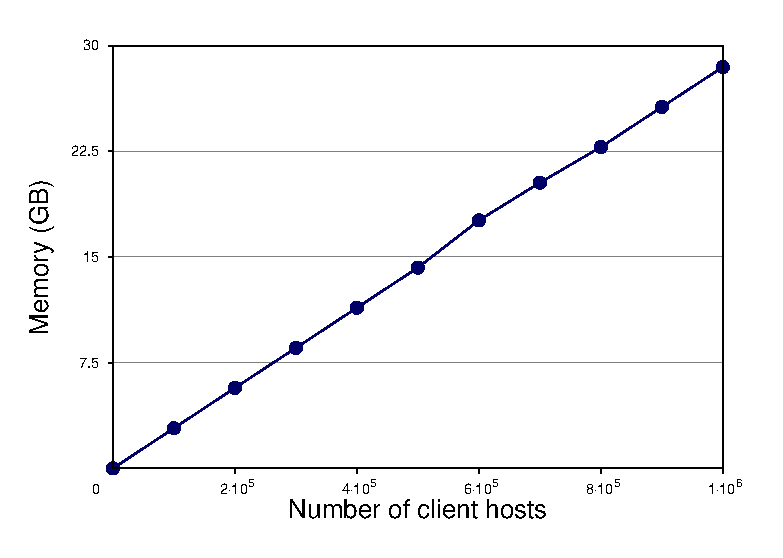
\includegraphics[width=\linewidth]{figures/memory}
		\caption{Memory usage.} 
		\label{fig:memory}
	\end{subfigure}
	\hspace*{\fill} % separation between the subfigures
	\begin{subfigure}{0.5\textwidth}
		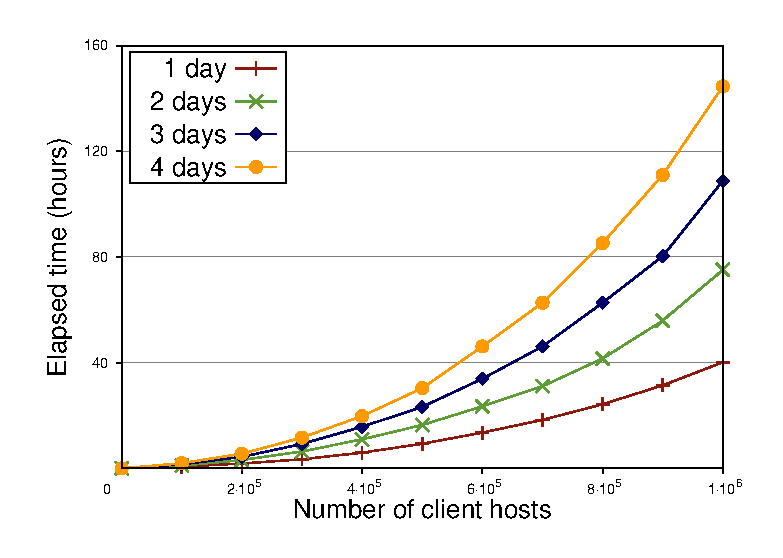
\includegraphics[width=\linewidth]{figures/time}
		\caption{Execution time.} 
		\label{fig:time}
	\end{subfigure}
	\caption{Performance study.}
	\label{fig:performance}
\end{figure}

\clearpage

\section{Case Studies}
\label{sec:case_studies}




\subsection{Combined Results}

